\documentclass[tikz]{standalone}
\usepackage{pgfplots}
\pgfplotsset{compat=1.18}
\begin{document}
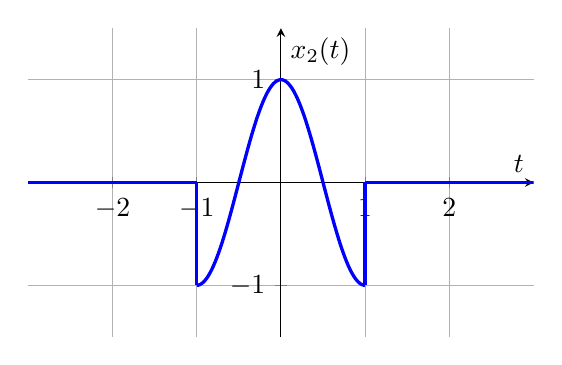
\begin{tikzpicture}
	\begin{axis}[
		width=8cm, height=5.5cm,
		axis lines=middle,
		xmin=-3, xmax=3, ymin=-1.5, ymax=1.5,
		xlabel={$t$}, ylabel={$x_2(t)$},
		grid=both,
		grid style={line width=.1pt, draw=gray!40},
		major grid style={line width=.2pt,draw=gray!60},
		xtick={-2,-1,0,1,2}, ytick={-1,0,1},
		samples=100
	]
	\addplot[line width=1.2pt, blue] coordinates {(-3,0) (-1,0)};
	\addplot[line width=1.2pt, blue, domain=-1:1, samples=100] {cos(deg(pi*x))};
	\addplot[line width=1.2pt, blue] coordinates {(-1,0) (-1,-1)};
	\addplot[line width=1.2pt, blue] coordinates {(1,-1) (1,0)};
	\addplot[line width=1.2pt, blue] coordinates {(1,0) (3,0)};
	\end{axis}
\end{tikzpicture}
\end{document}
